\section{Model-based Agent}
\label{sec:rlopt:subsec:mb-agent}
Unlike model-free reinforcement learning, in the domain of model-based reinforcement learning we aim to learn a model of the environment such that we no longer need the real simulator, providing numerous benefits such as improved sample efficiency, ability to plan trajectories of actions forward in time and decreased training time for systems environments. The primary task is model-based RL is to learn a model of the environment. Concretely, we aim to learn a function $f(z_t, a_t)$ that predicts the latent next state $z_{t+1}$ based on the action $a_t$ being performed in the state $z_t$, the reward $r_t$ and the terminal flag $d_t$ which indicates the end of the trajectory. Many environments, especially systems tasks, state transitions are stochastic and we must accurately represent such transitions in order to have a useful world model for planning. This section will further discuss how we designed the world model for learning the environment behaviour.

\subsection{World Models}
World models, introduced by Ha et al. \cite{ha2018worldmodels}, create an imagined model of the true environment by observing sequences of states, actions and rewards from the environment and learning to estimate the transitions between states based upon the actions taken. Ha et al. showed that the world models can learn the environment transitions and achieve state-of-the-art results on visual learning tasks such as CarRacing and VizDoom. One should note that Ha \& Schmidhuber used  a latent space embedding from the convolutional neural network based on the RGB pixel image; in this work we instead use the latent space produced by the graph neural network - in either case, we are learning the world model using the latent space of the environment. World models are constructed from three components. The ``visual'' module, taking the raw state from the environment and transforming into latent space, as well as the ``memory''  and ``controller`` modules which are discussed below.

[TODO include the world model algo w loss function?]

\subsubsection{Mixture Density Networks}
Mixture Density Networks (MDNs) are a class of network that can learn to output parameters to a probabilistic Gaussian mixture model (GMMs) \cite{bishop1994mixture}. A GMM is a function that is composed of several gaussians, each given a label $k \in \lbrace 1, \ldots, K \rbrace$, where $K$ is the number of components. Each gaussian is formed from three parameters $\mu_i$, the mean of component $i$, $\sigma_i$ the variance of component $i$ and $\pi$ the mixing probability/weight of each component. Unlike the networks used in supervised learning tasks that are trained using regression, training a GMM instead attempts to maximise the likelihood that the gaussians fit the data points in each minibatch. Inside a world model we use the predictions of an MDN at time $t$ to choose the parameters of the gaussian distribution for the next latent vector at time $t+1$. Notably, one can either use expectation maximisation to find the parameters of the model, or alternatively, can use a parameterised GMM which is trained in conjunction with the RNN using stochastic gradient descent.


\subsubsection{Recurrent Neural Networks}
\label{sec:rlopt:subsec:rnn}

Recurrent Neural networks (RNNs) are a class of architectures in which the connections between the nodes form a directed graph in a temporal sequence \cite{650093}. There are many forms which an RNN can take, each providing features and levels of stability which one many find useful for the task at hand. Importantly, the output of an RNN is deterministic, however, we can use the outputs from the RNN as the parameters for a probabilistic model to insert a controllable level of stochasticity in the output predictions \cite{graves2014generating}.

\begin{figure}[ht]
  \centering
  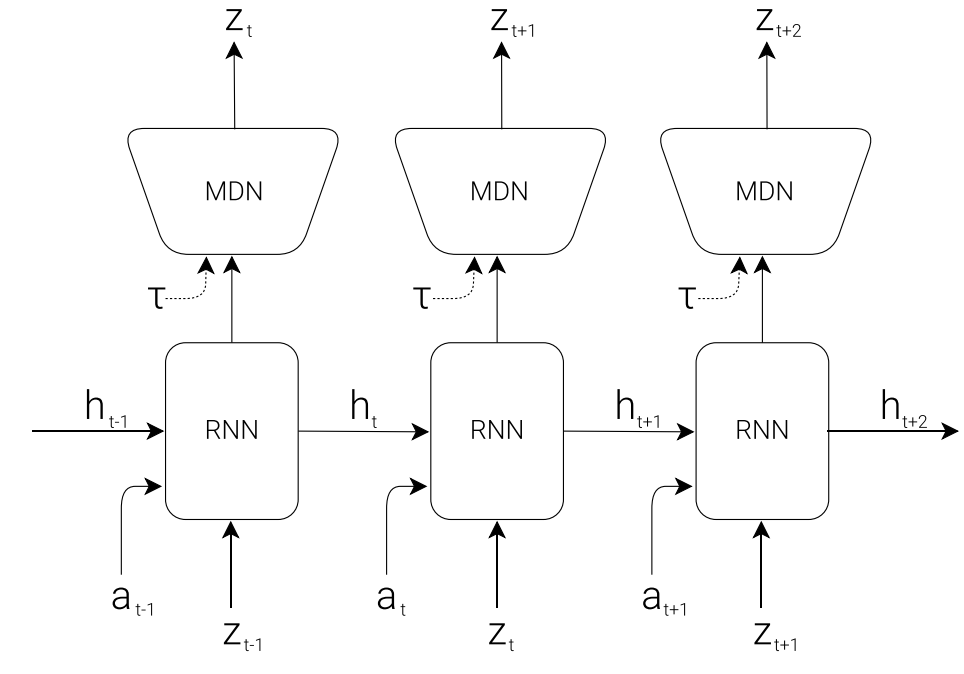
\includegraphics[width=0.75\columnwidth]{sections/4rlopt/images/mdnrnn.png}
  \caption[Temporally unrolled MDN-RNN]{Structure of an unrolled MDN-RNN. The MDN outputs the parameters of a Gaussian mixture distribution used to sample a prediction of the next latent vector $z_{t+1}$, the MDN is controlled by the temperature parameter $\tau$.}
  \label{fig:rl:mdnrnn}
\end{figure}

A constraint of using RNNs is that they expect a fixed sized input sequence. However, in our work, both the shape of the latent state tensor, and the number of actions performed by the agent in a rollout is variable. As such, we employ a common approach to mitigate this problem is by prepending zero values to the input sequence until the desired length is reached, commonly referred to as padding. After performing inference on the model and retrieving the predicted state, we mask the results based on the input padding to ensure we only use valid predictions to select the next action using the controller.

\subsubsection{MDN-RNN}

By combining the mixture density and recurrent networks, we can use rollouts of the environment sampled using a random agent to train the combined network, called an MDN-RNN. We use the network to model $P(z_{t+1}~|~a_t, z_t, h_t)$, where $z_t$, $z_{t+1}$ is the latent state at the times $t$ and $t+1$ respectively, $a_t$ is the action taken at time $t$, and $h_t$ is the hidden state from the RNN network at time $t$. Figure \ref{fig:rl:mdnrnn} shows the combination of the RNN and MDN networks and how we calculate the predictions of the next latent state in sequence.

Furthermore, after training the world model, we must train an agent (or controller) to perform actions in the world model and learn to take optimal actions that maximise reward. During inference of the world model, we use a softmax layer which outputs $\pi$ in the form of a categorial probability distribution which we sample under the Gaussian model parameterised by $(\mu_i, \sigma_i)$.

In figure \ref{fig:rl:mdnrnn} we show that one of the inputs to the MDN is $\tau$, the temperature. By altering the temperature it allows us to control the stochasticity of the agent during training of the controller. The logits of the RNN that represent the predictions for the values of $\pi$ are divided by the temperature prior to being passed into the softmax function which converts the logits into pseudo-probabilities. We incorporate the temperature, $\tau$, into the function using the following equation.

$$
\text{softmax}(\mathbf{x}_i) = \frac{\exp\left( \nicefrac{x_i}{\tau} \right) }{\Sigma_j \exp \left( \nicefrac{x_j}{\tau} \right) }
$$

Typically, temperature is a real number in the range $\tau \in \left[ 0, 1 \right)$, where a value of zero leads to completely deterministic predictions generated by the RNN, whereas larger values introduces a greater amount of stochasticity in the predictions. As larger values of $\tau$ increases the probability of samples with a lower sampling likelihood being selected it leads to a greater diversity of actions taken by the agent in the environment. Importantly, Ha et al. \cite{ha2018worldmodels} found that having a large temperature can aid in preventing the agent from discovering strategies to exploit in the world model which are not possible in the real environment due to imperfections in the model.

Modifying the softmax activation function in this way is equivalent to performing knowledge distillation between two models; learnt information is transferred from a large teacher model, or ensemble model, to a smaller model which acts as a student model. In both the context of knowledge distillation and training a controller actor inside the world model, a high temperature will generate a softer targets. Specifically, in this work a higher temperature produces a softer pseudo-probability distribution for $\pi$ in the GMM. Additionally, using soft targets will provide a greater amount of information for the model to be learn by forcing the model to learn more aggressive policies, thus outputting stochastic predictions which is beneficial to encourage exploring the environments state-action space.

Furthermore, we consider how the world model is trained. For any supervised learning task we require target data to which we can compare our predictions, calculate a loss and perform backpropagation to update the weights in the network. To train the world model, we use a random agent, one that has an equal probability of choosing any action from the valid set of actions in a given state. Unlike Ha and Schmidhuber \cite{ha2018worldmodels} who performed 10,000 rollouts of the environment offline using a random policy to collect the data, we took a slightly different approach. Instead, we generated minibatch rollouts using the random agent online, and directly used the observations to train the world model. Although this approach reduces the data efficiency as we only use each state observation once, we benefit from removing the need to generate the data prior to training. In systems environments, it is often expensive---in terms of computation time---to step the environment collect a diverse dataset. Therefore, we found generating short rollouts and training on the minibatch was beneficial without any perceivable impact on performance.

\subsection{Action Controller}
\label{sec:rlopt:subsec:actionctrl}

Finally, we discuss the design of the ``controller'', the network/agent that learns to output actions based upon the output from the MDN-RNN world model. Ha and Schmidhuber \cite{ha2018worldmodels} used an evolution based controller defined as a simple multi-layer-perceptron, $a_t = W_c[z_t, h_t] + b_c$, that accepts the hidden and current states from the recurrent network to predict the next action to be taken. A challenge when training the controller inside the fully imagined world environment is that we no longer have access to the ground truth state nor the reward produced by the real environment, therefore, we cannot use supervised learning to train the controller. 

In \cite{ha2018worldmodels} the authors used an evolutionally algorithm, covariance matrix adoption evolution strategy (CMA-ES) \cite{hansen2001completely, hansen2016cma}, which optimises the weights of the network based on the reward produced by the world model. Alternatively, recent work by Hafner et al. \cite{hafner2020dream, hafner2021mastering} has shown to achieve state-of-art results in the Atari environment using an actor-critic method as the controller in the world model. Furthermore, prior work on the application of world models to systems environments has shown one can train a model-free controller inside the world environment \cite{app10196685}.

% We also note that compared to previous work on training controllers inside a world model, the action space in this case is far larger than prior work. For example, in the simple case of CarRacing \cite{ha2018worldmodels}, there are only two possible actions. Similarly, in Atari \cite{hafner2021mastering}, there are between 

In our work, we use PPO, an on-policy algorithm which uses the world model state, rewards and terminal flags to optimise the control policy. Although any controller, from an shallow MLP to model-free RL algorithms can be used, the PPO algorithm is shown to be extremely robust to a range of parameters. For our work, we used the same algorithm to train the agent inside the real environment and in the world model, thus, acting as a good point of comparison for performance of the two methods. We show the results for training the model-free and model-based controllers in sections \ref{sec:eval:subsec:mfagent} and \ref{sec:eval:subsec:mbagent} respectively.

% {\SetAlgoNoLine
\begin{algorithm}[H]
\setstretch{1.0}
 Gather $N$ rollouts to form a dataset $\mathcal{D}_\text{RAND}$ of trajectories using random actions \\
 \For{k = 0, \dots, max\textunderscore iter}{
  Fit $\hat{f}_\theta (\mathbf{s}, \mathbf{a})$
 }
 \caption{Model-based Reinforcement Learning}
 \label{algo:mbrl}
\end{algorithm}}